A number of hazard calculation demos are provided with the \gls{acr:oqe}
installation,showing different examples of input and configuration files,
for different use cases.

This is the list of demos which illustrate how to use the \gls{acr:oqe} for
various seismic hazard analysis:

\begin{itemize}

    \item AreaSourceClassicalPSHA
    \item CharacteristicFaultSourceCase1ClassicalPSHA
    \item CharacteristicFaultSourceCase2ClassicalPSHA
    \item CharacteristicFaultSourceCase3ClassicalPSHA
    \item ComplexFaultSourceClassicalPSHA
    \item Disaggregation
    \item EventBasedPSHA
    \item LogicTreeCase1ClassicalPSHA
    \item LogicTreeCase2ClassicalPSHA
    \item LogicTreeCase3ClassicalPSHA
    \item PointSourceClassicalPSHA
    \item SimpleFaultSourceClassicalPSHA

\end{itemize}

\section{Classical PSHA Demos}
\label{sec:demos_classical_psha}
A number of demos have been designed to show how to perform a classical PSHA
calculation using the different available source typologies and how to define
non-trivial logic trees. It should be  noted that the input files that will be
illustrated are valid not only for a classical PSHA calculation but also for
event based and  disaggregation analysis.

All the classical PSHA demos illustrating the different source typologies (all
demos but the ones about Logic Tree definition) share the same GSIM logic tree
file, which for clarity is provided below in
Listing~\ref{lst:input_gmlt_demo}.

Since this logic tree consideres only one tectonic region (i.e. \texttt{Active
Shallow Crust}) all the seismic sources will belong be considered active
shallow crust sources.

\begin{listing}[htbp]
  \inputminted[firstline=1,firstnumber=1,fontsize=\footnotesize,frame=single,linenos,bgcolor=lightgray]{xml}{oqum/hazard/verbatim/input_gmlt.xml}
  \caption{GSIM logic tree input file used in the demos}
  \label{lst:input_gmlt_demo}
\end{listing}

\subsection{Classical PSHA with different source typologies}

This section discusses the following examples:

\begin{itemize}
    \item AreaSourceClassicalPSHA
    \item CharacteristicFaultSourceCase1ClassicalPSHA
    \item CharacteristicFaultSourceCase2ClassicalPSHA
    \item CharacteristicFaultSourceCase3ClassicalPSHA
    \item ComplexFaultSourceClassicalPSHA
    \item PointSourceClassicalPSHA
    \item SimpleFaultSourceClassicalPSHA
\end{itemize}

The configuration file in Listing~\ref{lst:config_classical} is defined to
compute hazard curves for several intensity measure types (PGV, PGA and
Spectral acceleration at different periods), hazard maps and uniform hazard
spectra for different probabilities of exceedance:

\begin{listing}[htbp]
  \inputminted[firstline=1,firstnumber=1,fontsize=\footnotesize,frame=single,linenos,bgcolor=lightgray,label=job.ini]{ini}{oqum/hazard/verbatim/config_classical.ini}
  \caption{Example configuration file for a classical probabilistic hazard calculation (\href{https://raw.githubusercontent.com/gem/oq-engine/master/doc/manual/oqum/hazard/verbatim/config_classical.ini}{Download example})}
  \label{lst:config_classical}
\end{listing}

Hazard maps for the different demos are shown in Figure~\ref{fig:hazard_maps1} and Figure~\ref{fig:hazard_maps2}.

\begin{figure}
\centering
\subcaptionbox{}
{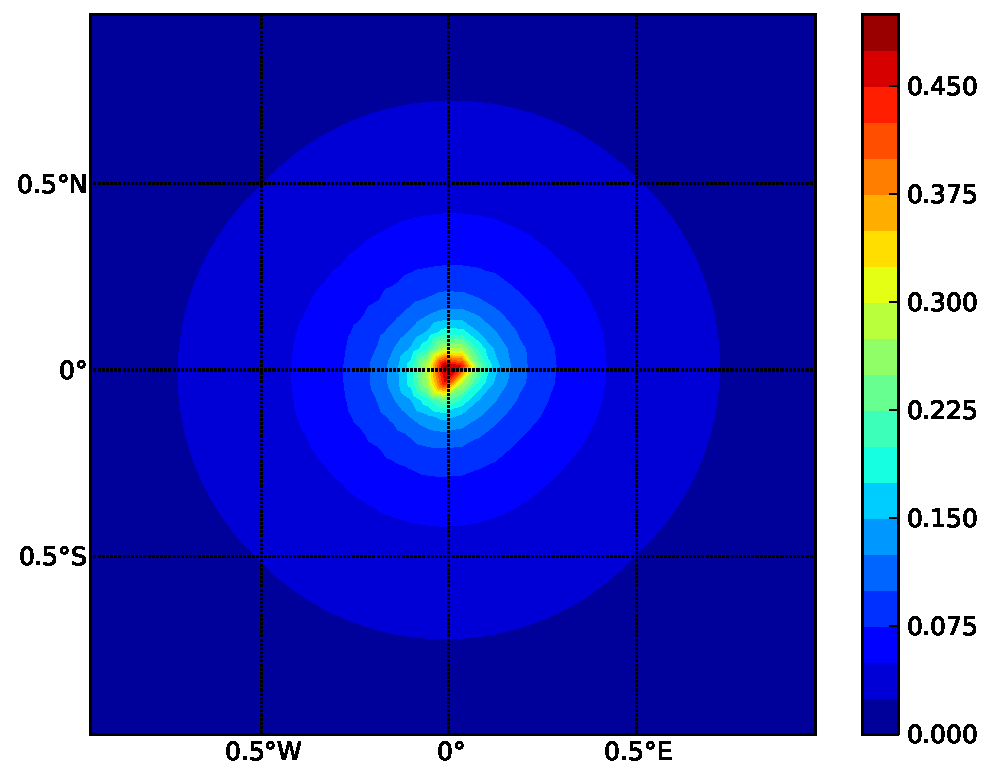
\includegraphics[width=7cm]{figures/hazard/point.pdf}}
\subcaptionbox{}
{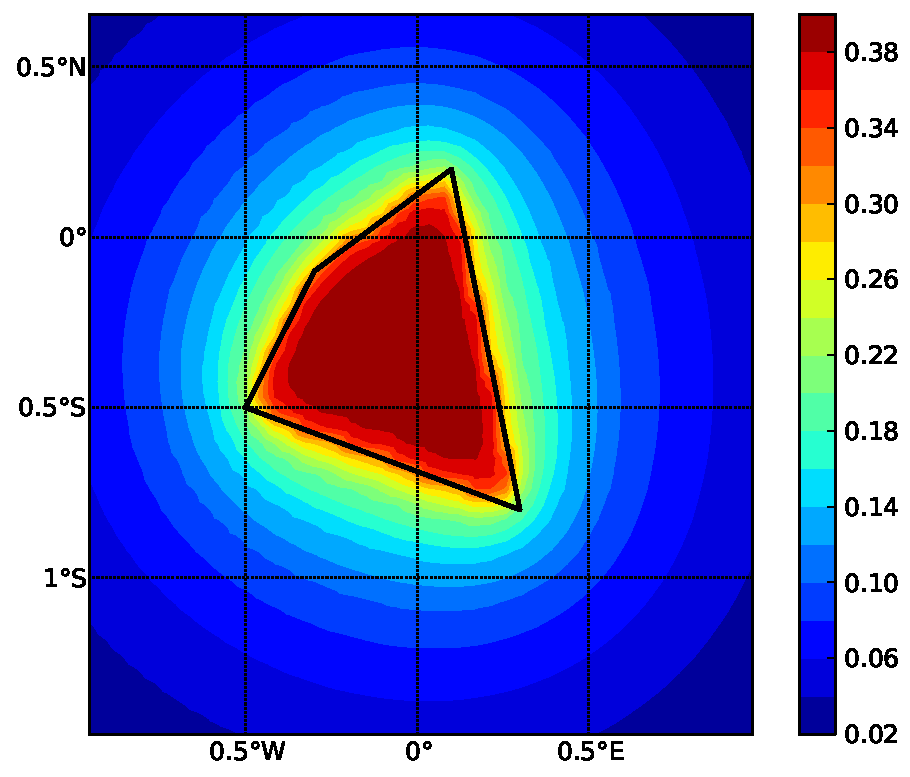
\includegraphics[width=7cm]{figures/hazard/area.pdf}} 
\subcaptionbox{}
{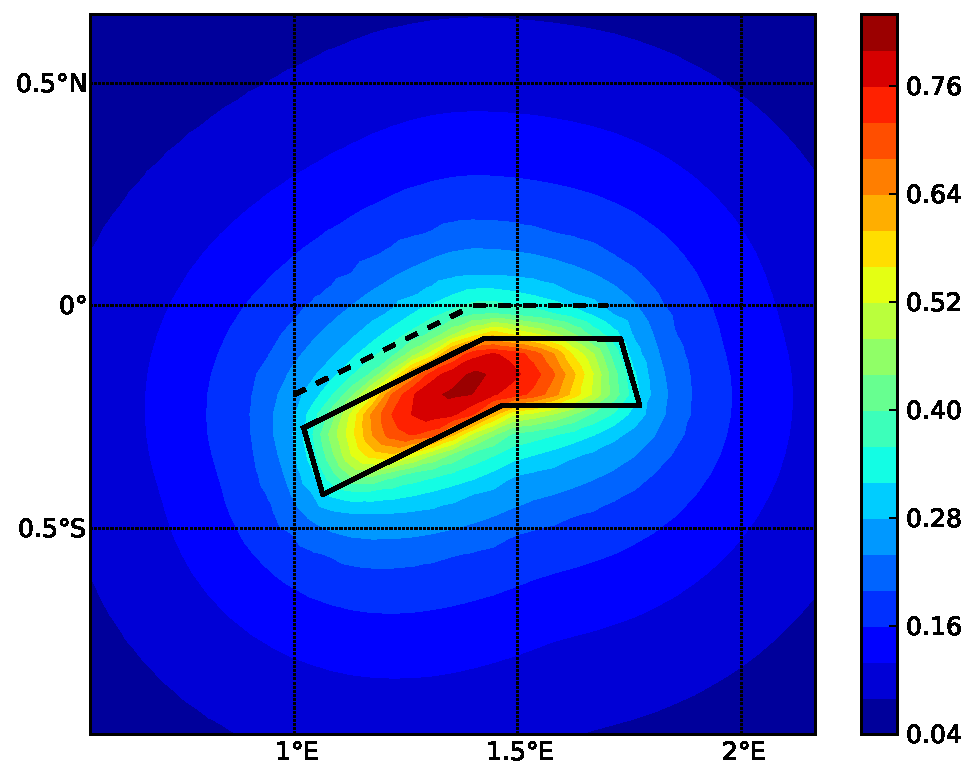
\includegraphics[width=7cm]{figures/hazard/simple_fault.pdf}} 
\subcaptionbox{}
{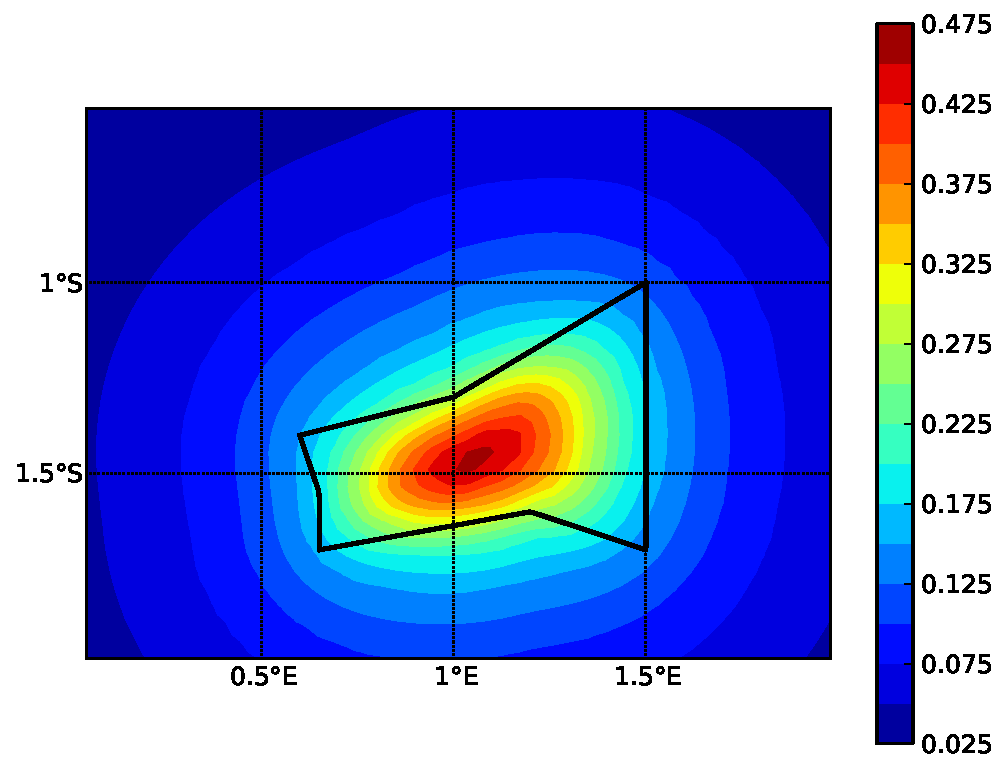
\includegraphics[width=7cm]{figures/hazard/complex_fault.pdf}} 
\caption{Hazard maps (for PGA, 10\% in 50 years) as obtained from the 
    different \gls{acr:oqe} source typologies. (a) Point Source. (b) Area 
    source.  The solid black line represents the area boundary. (c) Simple 
    Fault Source. 
    The dashed line represents the fault trace, while the solid line the fault
    surface projection. (d) Complex Fault Source. The solid line represent the 
    fault surface projection (d)}
\label{fig:hazard_maps1}
\end{figure}

\begin{figure} 
\centering 
\subcaptionbox{}
{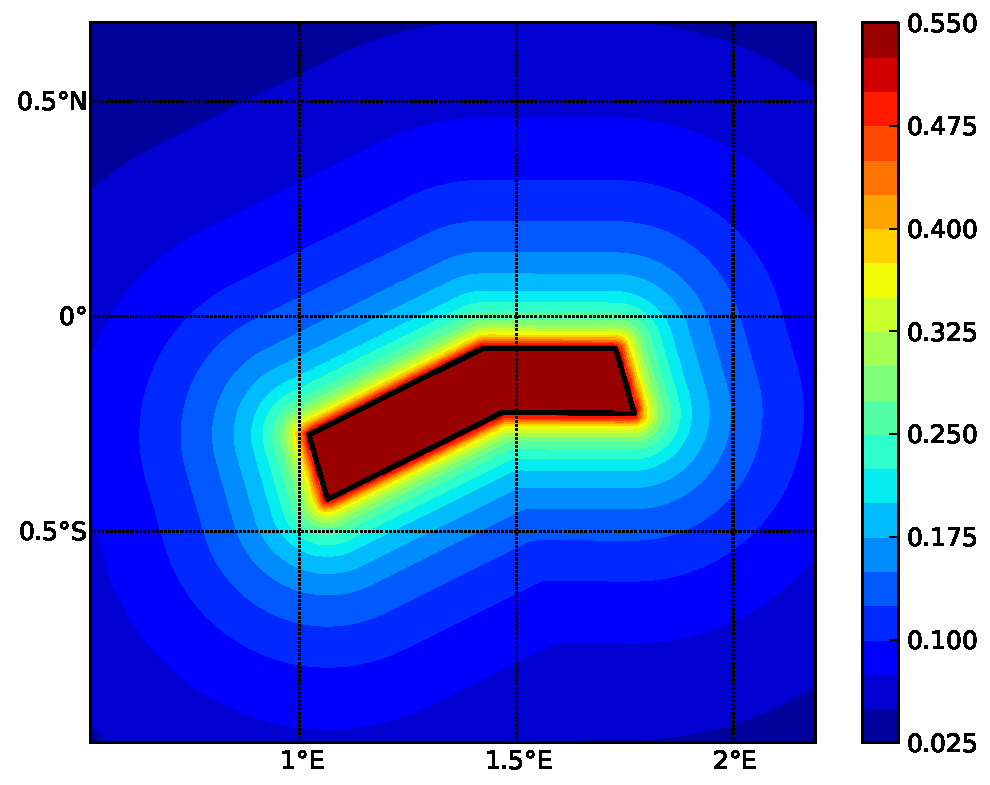
\includegraphics[width=7cm]{figures/hazard/char_fault2.pdf}} 
\subcaptionbox{}
{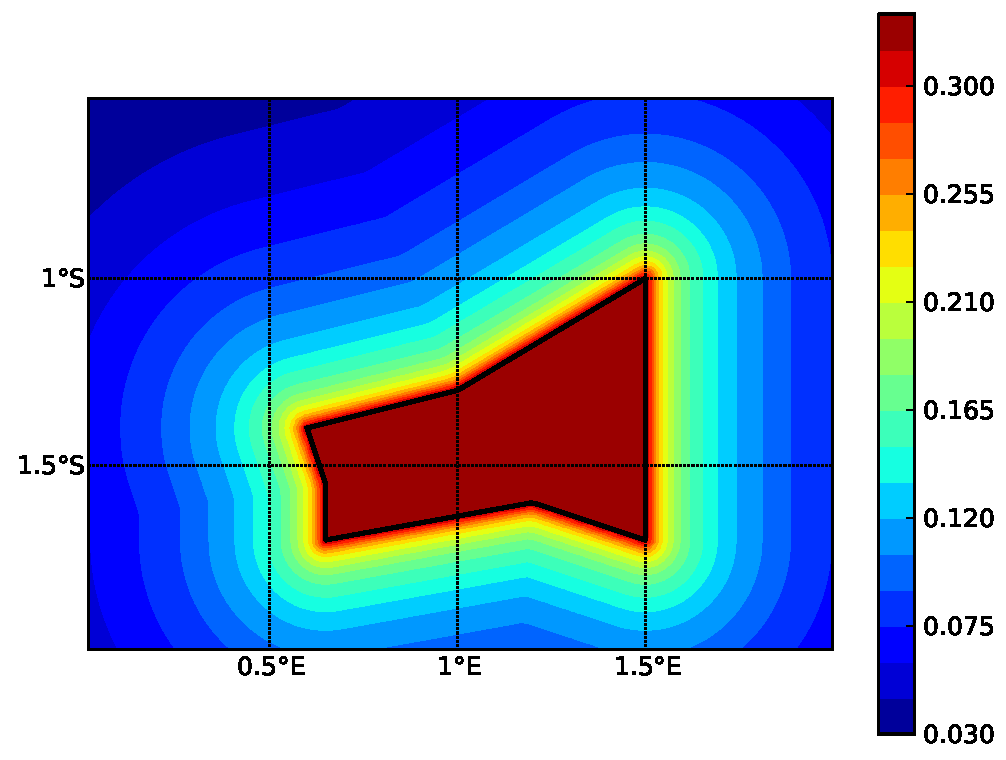
\includegraphics[width=7cm]{figures/hazard/char_fault3.pdf}} 
\subcaptionbox{}
{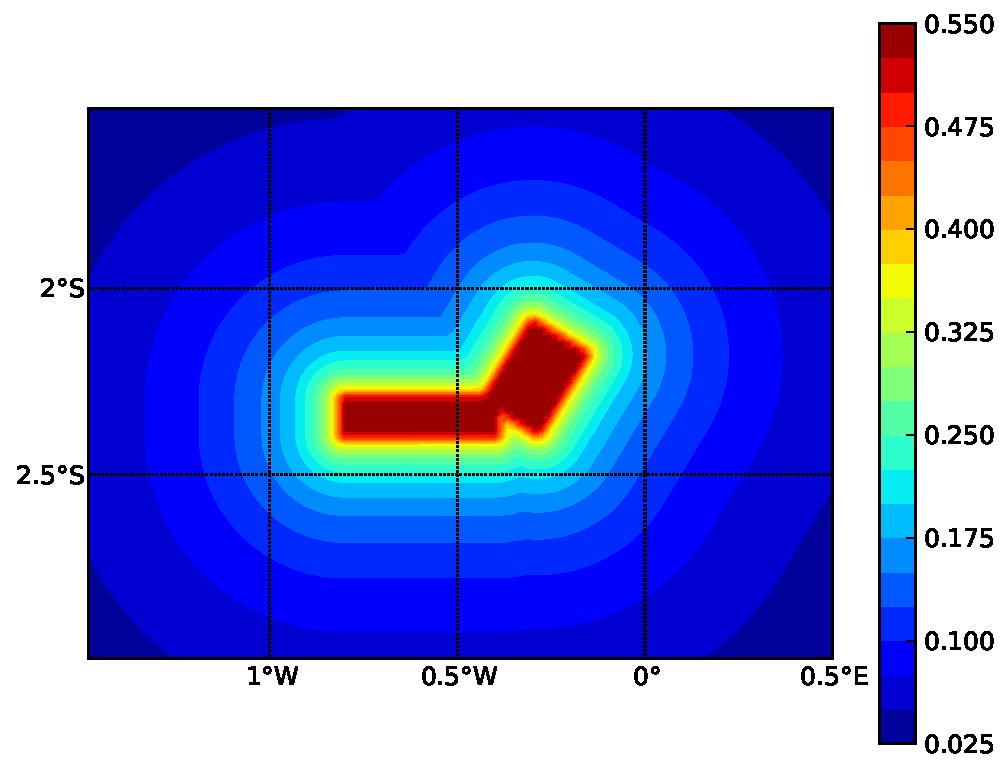
\includegraphics[width=7cm]{figures/hazard/char_fault1.pdf}} 
\caption{Hazard maps (for PGA, 10\% in 50 years) as obtained from 
    characteristic fault sources with simple fault
    geometry (a), complex fault geometry (b), and collection of
    planar surfaces (c)}
\label{fig:hazard_maps2}
\end{figure}

\clearpage
\subsection{Classical PSHA with non trivial logic trees}

Three demos are provided to illustrate how the logic tree formalism can be
used to express epistemic uncertainties in seismic hazard analysis.

LogicTreeCase1ClassicalPSHA shows an example of logic tree defining two
alternative source models, with sources belonging to two different tectonic
region types, and with two alternative GMPEs for each tectonic  region type.
The source model logic tree is therefore defined as shown in
Listing~\ref{lst:input_sslt_demo_LogicTreeCase1ClassicalPSHA}.

\begin{listing}[htbp]
  \inputminted[firstline=1,firstnumber=1,fontsize=\footnotesize,frame=single,linenos,bgcolor=lightgray]{xml}{oqum/hazard/verbatim/input_sslt_demo_LogicTreeCase1ClassicalPSHA.xml}
  \caption{Source model logic tree input file used in the LogicTreeCase1ClassicalPSHA demo}
  \label{lst:input_sslt_demo_LogicTreeCase1ClassicalPSHA}
\end{listing}

The two source models are defined in two separate files:
\texttt{source\_\-model\_\-1.xml} and \texttt{source\_\-model\_\-2.xml} each
one associated to a corresponding weight (0.5 for both).

The GSIM logic tree file contains the structure as shown in
Listing~\ref{lst:input_gmlt_demo_LogicTreeCase1ClassicalPSHA}.

\begin{listing}[htbp]
  \inputminted[firstline=1,firstnumber=1,fontsize=\footnotesize,frame=single,linenos,bgcolor=lightgray]{xml}{oqum/hazard/verbatim/input_gmlt_demo_LogicTreeCase1ClassicalPSHA.xml}
  \caption{GSIM logic tree input file used in the LogicTreeCase1ClassicalPSHA demo}
  \label{lst:input_gmlt_demo_LogicTreeCase1ClassicalPSHA}
\end{listing}

The source model contains sources belonging to Active Shallow Crust and
Stable Continental Crust, therefore the GSIM logic tree defines two branching
levels, one for each considered tectonic region type. Moreover for each
tectonic region a branch set with two GMPEs is defined: Boore and Atkinson
2008 and Chiou and Youngs 2008 for Active Shallow Crust and Toro et al. 2003
and Campbell 2003 for Stable Continental Crust. By processing the above logic
tree files using the logic tree path enumeration mode (enabled by setting in
the configuration file \texttt{number\_\-of\_\-logic\_\-tree\_\-samples = 0})
hazard results are computed for 8 logic tree paths (2 source models x 2 GMPEs
for Active x 2 GMPEs for Stable).

LogicTreeCase2ClassicalPSHA defines a single source model consisting of only
two sources (area and simple fault) belonging to different tectonic region
types (Active Shallow Crust and Stable Continental Region) and both
characterized by a truncated Gutenberg-Richter distribution. The logic tree
defines uncertainties for G-R a and b values (three possible pairs for each
source), maximum magnitude (three values for each source) and uncertainties
on the GMPEs for each tectonic region type (two GMPE per region type).

To accommodate such a structure the GSIM logic tree is defined as shown in
Listing~\ref{lst:input_gmlt_demo_LogicTreeCase2ClassicalPSHA}.

\begin{listing}[htbp]
  \inputminted[firstline=1,firstnumber=1,fontsize=\footnotesize,frame=single,linenos,bgcolor=lightgray]{xml}{oqum/hazard/verbatim/input_gmlt_demo_LogicTreeCase2ClassicalPSHA.xml}
  \caption{GSIM logic tree input file used in the LogicTreeCase2ClassicalPSHA demo}
  \label{lst:input_gmlt_demo_LogicTreeCase2ClassicalPSHA}
\end{listing}

The first branching level defines the source model. For each source, two
branching levels are created, one defining uncertainties on G-R a and b values
(defined by setting \texttt{uncertaintyType="abGRAbsolute"}) and G-R maximum
magnitude (\texttt{uncertaintyType="maxMagGRAbsolute"}).

It is important to notice that each branch set is applied to a specific source
by defining the attribute \texttt{apply\-To\-Sources}, followed by the source
ID. The GSIM logic tree file is the same as used for
LogicTreeCase1ClassicalPSHA. By setting in the configuration file
\texttt{number\_\-of\_\-logic\_\-tree\_\-samples = 0}, hazard results are
obtained for 324 paths (1 source model x 3 (a, b) pairs for source 1 x 3 (a,
b) pairs for source 2 x 3 max magnitude values for source 1 x 3 max magnitude
values for source 2 x 2 GMPEs for Active Shallow Crust X 2 GMPEs for Stable
Continental Crust), see Figure~\ref{fig:hazard_curves}.


\begin{figure}
\centering
\subcaptionbox{}
{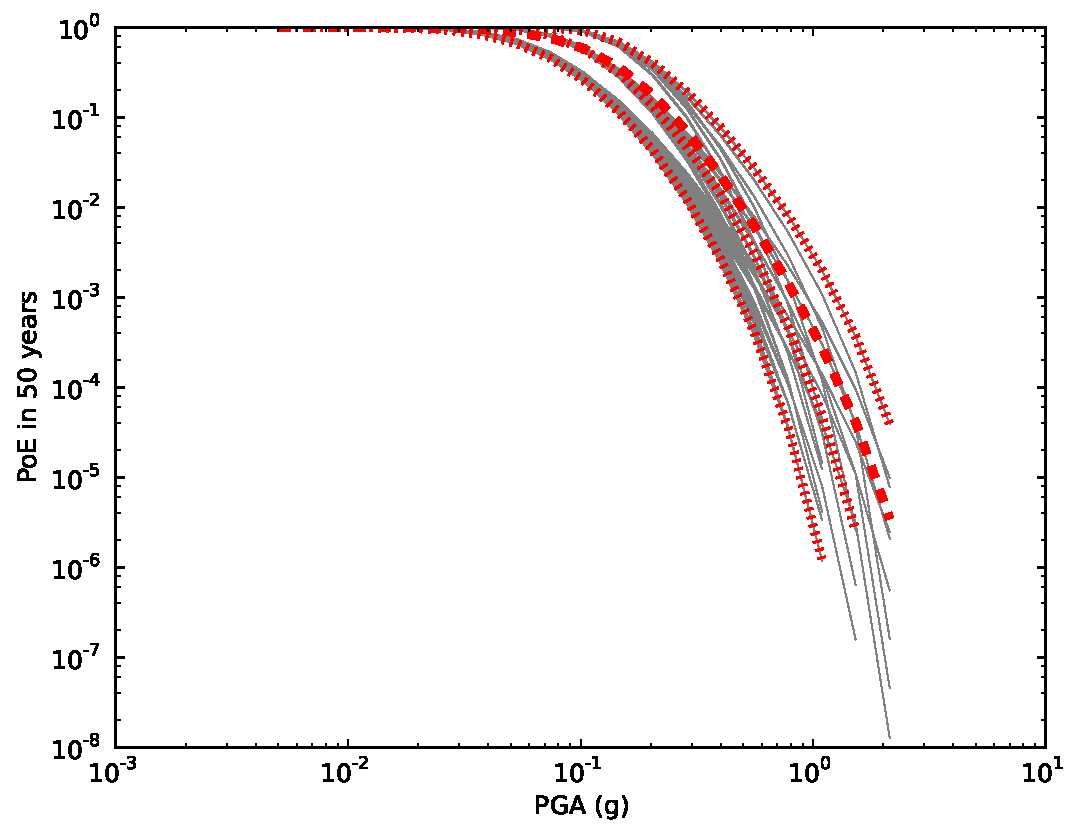
\includegraphics[width=9cm]{figures/hazard/hazard-curves-ltcase2.pdf}} 
\caption{Hazard curves as obtained from the LogicTreeCase2 demo. Solid gray 
    lines represent individual hazard curves from the different
    logic tree path (a total of 324 curves). The red dashed line represents the
    mean hazard curve, while the red dotted lines depict the quantile levels
    (0.15, 0.5, 0.95).}
\label{fig:hazard_curves}
\end{figure}

LogicTreeCase3ClassicalPSHA illustrates an example of logic tree defining
relative uncertainties on G-R maximum magnitude and b value. A single source
model is considered containing two sources belonging to different tectonic
region types and both characterized by a G-R magnitude frequency distribution.
The source model logic tree for this demo is as shown in
Listing~\ref{lst:input_sslt_demo_LogicTreeCase3ClassicalPSHA}.

\begin{listing}[htbp]
  \inputminted[firstline=1,firstnumber=1,fontsize=\footnotesize,frame=single,linenos,bgcolor=lightgray]{xml}{oqum/hazard/verbatim/input_sslt_demo_LogicTreeCase3ClassicalPSHA.xml}
  \caption{Source model logic tree input file used in the LogicTreeCase3ClassicalPSHA demos}
  \label{lst:input_sslt_demo_LogicTreeCase3ClassicalPSHA}
\end{listing}

After the first branching level defining the source model, two additional
branching levels are defined, one defining relative uncertainties on b value
(\texttt{bGRRelative} applied consistently to all sources in the source
model) and the second uncertainties on maximum magnitude
(\texttt{maxMagGRRelative}). Similar to the other cases, two GMPEs are
considered for each tectonic region type and therefore the total number of
logic tree path is 36 (1 source model x 3 b value increments x 3 maximum
magnitude increments x 2 GMPE for Active x 2 GMPEs for Stable).

\section{Hazard Disaggregation Demos}
\label{sec:demos_hazard_disaggregation}
An example of disaggregation calculation is given considering a source model
consisting of two sources (area and simple fault) belonging to two different
tectonic region types.

The calculation is defined with the following configuration file:

\begin{Verbatim}[frame=single, commandchars=\\\{\}, fontsize=\normalsize]
[general]
description = ...
calculation_mode = disaggregation
random_seed = 23

[geometry]
sites = 0.5 -0.5

[logic_tree]
number_of_logic_tree_samples = 0

[erf]
rupture_mesh_spacing = 2
width_of_mfd_bin = 0.1
area_source_discretization = 5.0

[site_params]
reference_vs30_type = measured
reference_vs30_value = 600.0
reference_depth_to_2pt5km_per_sec = 5.0
reference_depth_to_1pt0km_per_sec = 100.0

[calculation]
source_model_logic_tree_file = source_model_logic_tree.xml
gsim_logic_tree_file = gmpe_logic_tree.xml
investigation_time = 50.0
intensity_measure_types_and_levels = {"PGA": [...]}
truncation_level = 3
maximum_distance = 200.0

[disaggregation]
poes_disagg = 0.1
mag_bin_width = 1.0
distance_bin_width = 10.0
coordinate_bin_width = 0.2
num_epsilon_bins = 3

[output]
export_dir = ...
\end{Verbatim}

Disaggregation matrices are computed for a single site (located between the
two sources) for a ground motion value corresponding to a probability value
equal to 0.1 (\texttt{poes\_\-disagg = 0.1}). Magnitude values are classified
in one magnitude unit bins (\texttt{mag\_\-bin\_\-width = 1.0}), distances in
bins of 10 km (\texttt{distance\_\-bin\_\-width = 10.0}), coordinates in bins
of 0.2 degrees (\texttt{coordinate\_\-bin\_\-width = 0.2}). 3 epsilons bins
are considered (\texttt{num\_\-epsilon\_\-bins = 3}).


\section{Event Based PSHA Demos}
\label{sec:demos_event_based_psha}
A demo showing an example of Event Based PSHA calculation is provided with the
following configuration file:

\begin{Verbatim}[frame=single, commandchars=\\\{\}, fontsize=\normalsize]
[general]
description = Event Based PSHA using Area Source
calculation_mode = event_based
random_seed = 23

[geometry]
sites = 0.5 -0.5

[logic_tree]
number_of_logic_tree_samples = 0

[erf]
rupture_mesh_spacing = 2
width_of_mfd_bin = 0.1
area_source_discretization = 5.0

[site_params]
reference_vs30_type = measured
reference_vs30_value = 600.0
reference_depth_to_2pt5km_per_sec = 5.0
reference_depth_to_1pt0km_per_sec = 100.0

[calculation]
source_model_logic_tree_file = source_model_logic_tree.xml
gsim_logic_tree_file = gmpe_logic_tree.xml
investigation_time = 50.0
intensity_measure_types_and_levels = {"PGA": [...]}
truncation_level = 3
maximum_distance = 200.0

[event_based_params]
ses_per_logic_tree_path = 100
ground_motion_correlation_model =
ground_motion_correlation_params =

[output]
export_dir = ...
ground_motion_fields = true
hazard_curves_from_gmfs = true
mean_hazard_curves = false
quantile_hazard_curves =
hazard_maps = true
poes = 0.1
\end{Verbatim}

The source model consist of one source (area). 100 stochastic event sets  are
generated (\texttt{ses\_\-per\_\-logic\_\-tree\_\-path = 100}) (an example
can be seen in Figure~\ref{fig:ses}). Ground motion fields are computed
(\texttt{ground\_\-motion\_\-fields = true}, Figure~\ref{fig:gmfs}) and also
hazard curves from ground motion fields are extracted
(\texttt{hazard\_\-curves\_\-from\_\-gmfs = true}). The corresponding hazard
maps for 0.1 probability are also calculated (\texttt{hazard\_\-maps = true})

\begin{figure}
\centering
\subcaptionbox{}
{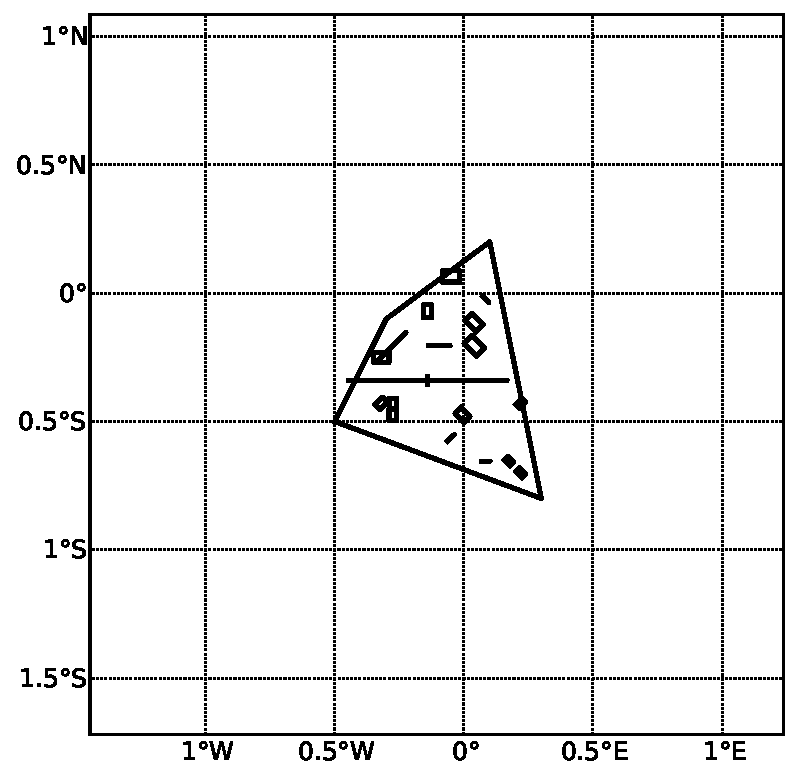
\includegraphics[width=9cm]{figures/hazard/ses.pdf}} 
\caption{A stochastic event set generated with the event based PSHA demo. 
    The area source defines a nodal plane distribution which distributes 
    events among vertical and dipping (50 degrees) faults with equal weights. 
    Vertical ruptures are then distributed equally in the range 0-180 degrees 
    while the dipping ones in the range 0-360, both with a step of 45 degrees.}
\label{fig:ses}
\end{figure}

\begin{figure}
\centering
\subcaptionbox{}
{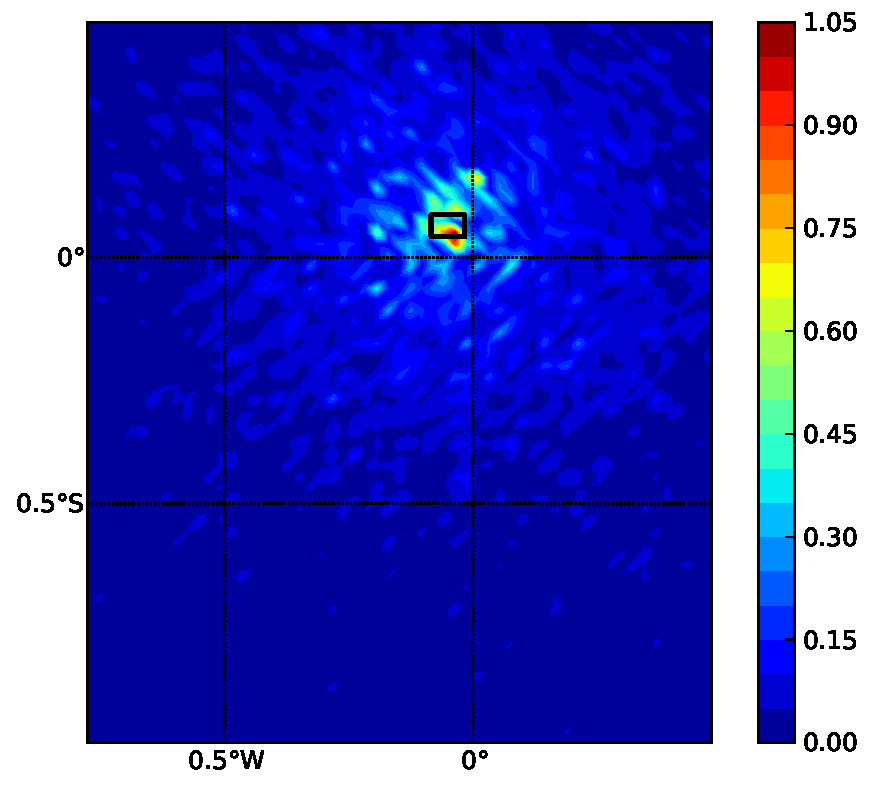
\includegraphics[width=6cm]{figures/hazard/gmf-no-corr.pdf}} 
\subcaptionbox{}
{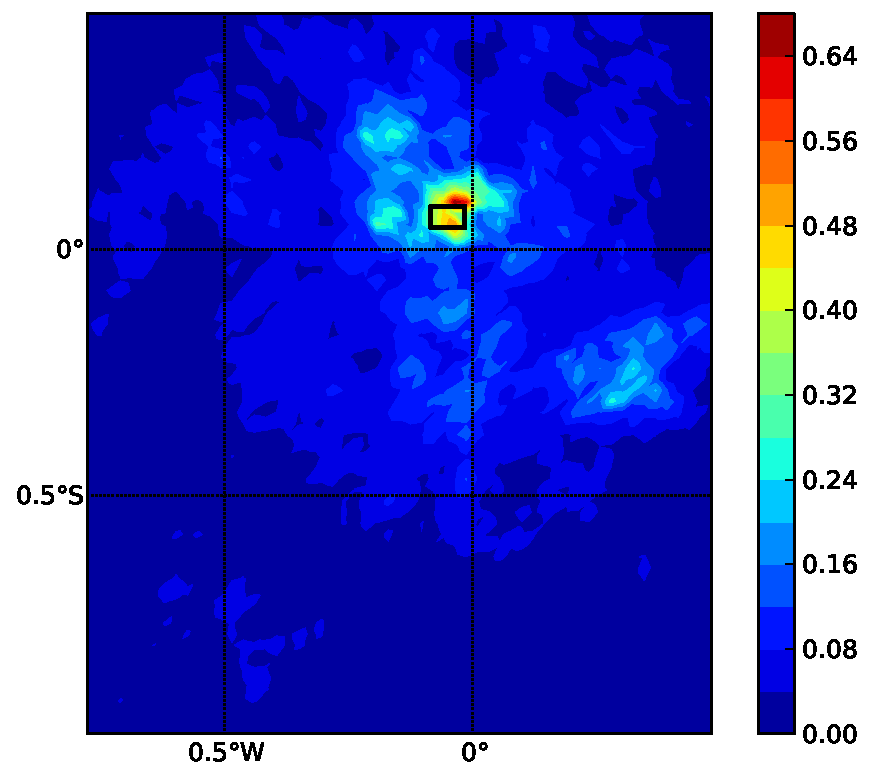
\includegraphics[width=6cm]{figures/hazard/gmf-corr.pdf}} 
\caption{Ground motion fields (PGA) with no spatial correlations (a) and with spatial correlation (b)}
\label{fig:gmfs}
\end{figure}

% \section{Scenario Hazard Demos}
% \label{sec:demos_scenario_hazard}
% \input{oqum/hazard/03d_scenario_demos}
